\section{Approach to the Study}

Several tasks are necessary for the project. One task is to implement
the algorithms for different models, one the sequence to sequence model
and the other the transformer model for a generative chatbot and finally the GPT2 model.

We will not try to rewrite the transformer or GPT2 model ourselves.

\section{Setup}

We use linux computers, sometimes with gpu hardware for parallel processing.
We also use the Python programming language. Code from this project
can be run with the 3.x version of Python.

When the project was started we did some programming with Keras using
Tensorflow as a backend. Keras was later discarded in favor of Pytorch.
Pytorch as a library is still under development at the time of this
writing.

Some of the GPT2 code uses Pytorch. Some of the Transformer and GPT2 code uses Tensorflow. There
is a repository on Github that has the GPT2 trained model using Pytorch instead of Tensorflow.

We use github as a code repository. Code corresponding with this paper
can be found at: \href{https://github.com/radiodee1/awesome-chatbot}{https://github.com/radiodee1/awesome-chatbot}
. 

As a coding experiment we rewrite the code for the sequence-to-sequence model. We have varying amounts of success with these experiments. We do not rewrite the GPT2 code from the Tensorflow or Pytorch repository.

\section{ARMv7 Build/Compile}

\subsection*{Pytorch `torch' Library 1.1.0 For ARMv7}
We compile the Pytorch library for Raspberry Pi. We use several virtualization techniques to do this compilation. The result of those efforts is a Pytorch python 3.7 library for the Raspberry Pi.

Explanation here.

\subsection*{Docker Container `tensorflow-model-server' For ARMv7}
Docker has to be installed on the Raspberry Pi and on the development laptop computer.

Then we use someone's pre-compiled Docker Container for ARMv7. We write our own Docker script to interact with the pre-compiled container.

Explanation here.

\section{Experiments}

We have several basic neural network models. One is the basic sequence
to sequence model typically used for neural machine translation. We also have the transformer and
the GPT2.

The GPT2 code is versatile. We use it for the chatbot problem. The GPT2 model
is pretrained. We experiment with transfer learning and further training of the GPT2 model, but
in our case it does not improve the model's performance. 

When we talk about the chatbot problem on GPT2 we are talking about a PyTorch version of the 
GPT2 code. 

We found that the chatbot with the hand coded Neural Machine Translation did not work 
very well. We found that the GPT2 chatbot worked well enough with the `zero-shot' setup so that
fine-tuning was not necessary. 

Fine tuning on the GPT2 problem actually had a negative effect. To fine-tune GPT2 also involved
training the model on Tensorflow and then translating the model to PyTorch when that was done. 

We use speech recognition and speech to text libraries to allow a user to give the chatbot model 
auditory input.

We also train the transformer to do the chatbot task. This works better than the sequence to 
sequence but not as well as the GPT2.

Finally we describe installing the chatbot in small computing platforms, the Raspberry Pi and the O-Droid, in an attempt to create a smart speaker.

All of the three mentioned models work on a laptop computer.

It should be noted that at some point we would like to describe some of our subjective
results with the different models. It is difficult to measure our results objectively because we
are using code most closely associated with a translation task. 

If we were measuring progress with an actual translation task accuracy could be measured as a score that improves when the output matches the meaning of the input, albeit in a different language. We don't use an actual translation
task, we use something close to one. The problem is that though the input 
and the output are in the same language, the input and output have different meanings. We
do not dictate what the correct output would be for a given input. The output just has to make sense as a reply in the English language. We would actually prefer that the output not have the
same meaning as the input. This makes it difficult to calculate an objective accuracy score. This
is touched on in the paper from Vinyals et al(2015)\cite{DBLP:journals/corr/VinyalsL15}.

Loss can still be monitored during training. When the loss stops decreasing you know you should 
stop training as the model is probably overfitting.

\iffalse
\begin{figure}[H]
	
	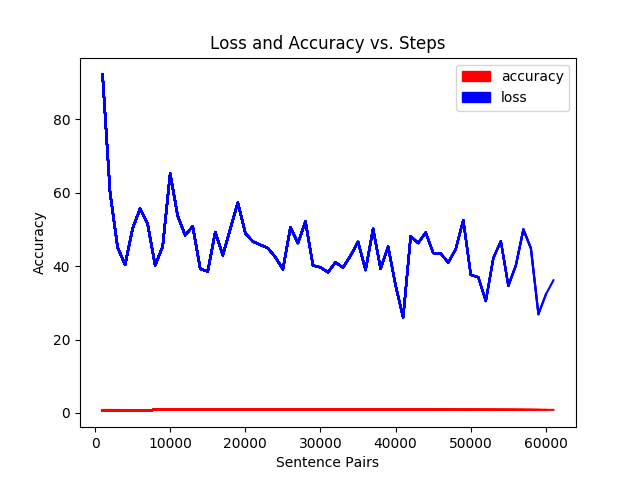
\includegraphics[scale=1.0]{Figure_1}
	
	\caption[Loss and Accuracy]{Loss and Accuracy: Red is accuracy and blue is loss.}
	
%\addcontentsline{lof}{section}{Loss and Accuracy}
\end{figure}
\fi

\section{Chatbot - GRU Model}
We trained the sequence to sequence model on a large english
corpus in an attempt to produce a chatbot. 

For the sequence to sequence model we want to use text found in a movie dialog corpus (Danescu-Niculescu-Mizil et al, 2011)\cite{Danescu-Niculescu-Mizil+Lee:11a}. 

In our experience with coding our own chatbot 
we find that the model learns a single english sentence that can be used for most replies. 

Subjectively the GRU chatbot is unusable.

For example our chatbot frequently replies to input with the phrase "I don't know". This is the most common output from our model. In this respect our original chatbot responds poorly.

A large portion of the time the bot's 
response to a question is "I don't know". This is interesting in that the chatbot has identified that this phrase is a suitable answer to many questions, but it is disappointing that there is not more variety to the output.  

Occasionally the sequence-to-sequence model will reply with the phrase "I'm sorry." This happens
very infrequently and it is not clear why the model chooses to reply this way. 

\section{Smart Speaker - GRU Model}

The GRU model was installed on a Raspberry Pi. This allowed us to test out speech-to-text and 
text-to-speech libraries. 

%\subsection*{Pytorch 'torch' Library 1.1.0 For ARMv7}
It also allowed us to compile the Pytorch library for Raspberry Pi.



\section{Chatbot - Transformer Model}
Using the Persona corpus we trained a transformer model to use as a chatbot. This transformer was not pre-trained with any large corpus, so this example did not use transfer learning. 

Subjectively this model did not perform as well as the GPT2 model, but it did perform better than the GRU model.

The memory footprint of the model while it was running was below 1 Gigabyte. It is conceivable that the model could be installed on a Raspberry Pi board but it requires a python package called `tensorflow-model-server' and this package would have to be built from source for the Raspberry Pi. 

Training of the model followed a certain pattern. First the model was trained on the persona corpus until a familiar pattern emerged. When the model began to answer all questions with the 
phrase "I don't know" training was stopped. 

At that time the corpus was modified to include no 
sentences that have the word "don't" in them. Training was started again until the output contained nothing but the phrase "I'm sorry." 

At that time the corpus was modified to include no sentences that have the word "sorry" in them.
Training was started again and was continued for some period. Training was stopped. A further segment of training was not attempted. 

At this point, after looking at the change in loss, further training was not
thought of as helpful. Loss stopped improving at some point in this process, and this lack of
improvement was taken as a sign that progress was not likely.

Subjectively the transformer model is better than the GRU model. It can respond to something like
four sentences. When it comes upon a question that it doesn't expect it defaults to a certain sentence. It can answer questions that you might ask in a rudimentary conversation. It has answers to prompts like `hi', `How are you?' and `What do you do?'. If you tell it your name it will tell you that its name is `Sarah'. It doesn't answer arbitrary questions. It cannot answer 'What is your favorite color?'. It cannot tell you the time. The default reply sentence for unknown prompts is `Hi, how are you today?'

\section{Smart Speaker - Transformer Model}

Later we look to install the transformer model on the Raspberry Pi. This model is more dynamic than the sequence-to-sequence model. 

The transformer model takes about two minutes to boot on the Raspberry Pi. After that the time between responses is slow. The time between the first two or three responses is uncomfortably slow. After those first responses the time between answers gets to be more natural.



\section{Chatbot - GPT2 Model}
We used a pre-trained GPT2 model with the large english corpus to produce a chatbot and ascertain if this model works better than the sequence-to-sequence model. In our tests this worked well. The corpus is called `WebText'.

For our experiments GPT2 was used for the chatbot model in `zero-shot' mode. This means we did no
special fine-tuning of the GPT2 model in the application.

We did do some special coding for the input and output of the GPT2 code in order to operate it as
a chatbot. Input and output was limited to about 25 tokens. 

Input to the model was prepended with the character string "Q:" by our code. Output was observed 
to have the character string "A:" prepended to it. We assume therefore that the GPT2 model was at some point
exposed to the "Question/Answer" paradigm in written passages during its training. This was helpful.

Output from the GPT2 model was 
usually larger in size than we needed. Also, output had the character of having some sensible utterance followed by some output that was only a partial sentence.

It was necessary to `scrape' the output. First the output was checked for the "A:" character string at the start. If it was there it was removed. Then the first complete sentence was used as output, while words and phrases after that were discarded.

Lastly we decided that we would attempt to give the model some details that it could draw on 
during normal execution. We had two choices here. One choice was to train the model using fine-tuning and transfer learning to recognize certain questions and to supply answers. The other
choice was to simply show the model the list of facts that we thought were important before 
every input sequence. This information would be summarized with each reply.

The second choice was more interesting. The text that the model was shown always included the name of 
the model (picked somewhat arbitrarily) along with information about the location of the model
and the occupation. The time was also included.

Subjectively the model was the best of the three tested. The model would answer questions about it's location, it's name, and the time, faithfully most
of the time. Interestingly there where times when it did not do so. Some times it used 
alternative answers. For example, it would answer with the time but not the correct time. This was odd.

Under almost all circumstances the output was sensible English. There were few if any times 
where the model replied with gibberish. 

The subject matter of the prompts did not need to be the
same as the simple introductory conversation of the transformer model. In fact any subject matter
could be chosen and the model would answer. The model did not remember its own answers but it
was consistent. Questions it answered include `What is your favorite color?' and `Do you like lollipops?'. 

\section{Smart Speaker - GPT2 Model}
Tests showed that the GPT2 chatbot worked well. We wanted to continue and allow the chatbot to
have more of the abilities of a smart speaker. We constructed a simple corpus that contained
key phrases that we wanted the chatbot to recognize and act upon. We did some transfer learning
with this new corpus.

We found that one of two things would happen. The chatbot would either learn the new phrases and forget all it's pre-training, or it would not learn the new phrases and it would retain all it's 
pre-training. For our examples there seemed to be no middle ground. Comparisons were made with 
all available models and a version without the transfer learning was settled on.

Code was added that uses Text To Speech and Speech To Text libraries. In this way the model could
interact with a subject using auditory cues and commands.

We did some programming that allowed the GPT2 model to launch programs when directed to by
the user. In this way we have tried to move our project closer to the smart-speakers that
are produced commercially. The programming did not rely on the neural-network aspects of the
model. Instead the code used heuristics and simple word recognition. This code can be disabled
when the model is run from the command line.


